\documentclass[letterpaper,11pt]{article}
\usepackage[top=1in, bottom=1in, left=1in, right=1in]{geometry}
\usepackage{subfiles}
\usepackage[T1]{fontenc}
\usepackage[sfdefault]{cabin}
\renewcommand{\familydefault}{\sfdefault}

\usepackage[utf8]{inputenc} % For UTF-8 encoding
\usepackage{amsmath}        % For mathematical typesetting
\usepackage{graphicx}       % For images
\usepackage{float}
\usepackage[hidelinks]{hyperref}
\usepackage{xcolor}
\usepackage{titlesec}
\usepackage{listings}
\usepackage{courier}
\usepackage[backend=biber,style=ieee]{biblatex}
\addbibresource{references.bib}
\usepackage{array}
\usepackage{booktabs}
\usepackage{multirow}
\usepackage{nameref}
\usepackage{circuitikz} % https://mirrors.ibiblio.org/CTAN/graphics/pgf/contrib/circuitikz/doc/circuitikzmanual.pdf
\usepackage{wrapfig} 
\usepackage{titling}

\usepackage{fancyhdr}  % For headers and footers
\pagestyle{fancy}      % Use fancy style

% Define header and footer
\fancyhead[L]{}    % Left header
\fancyhead[C]{Circuits \& Code: Mastering Embedded Co-op Interviews}  % Center header (optional)
\fancyhead[R]{}   % Right header

%\fancyfoot[L]{Advance Review Copy} 
\fancyfoot[C]{Page \thepage}       
%\fancyfoot[R]{DO NOT DISTRIBUTE}    
\fancyfoot[R]{\bluehref{https://circuits-and-code.github.io}{circuits-and-code.github.io}}      

% Remove default header/footer rule lines if needed
\renewcommand{\headrulewidth}{0.4pt}  % Header line thickness (0pt removes it)
\renewcommand{\footrulewidth}{0.4pt}  % Footer line thickness (0pt removes it)

% Listings settings for C language
\lstdefinestyle{modernC}{
    language=C,
    basicstyle=\ttfamily\small, % Use modern monospaced font
    keywordstyle=\color{blue}\bfseries,
    identifierstyle=\color{black},
    commentstyle=\color{gray}\itshape,
    stringstyle=\color{teal},
    numberstyle=\tiny\color{gray},
    numbers=left, 
    numbersep=8pt,
    backgroundcolor=\color{gray!10}, % Light gray background
    frame=single,
    tabsize=4,
    captionpos=b,
    breaklines=true,
    showstringspaces=false,
    escapeinside={\%*}{*)}, % Escaping for inline LaTeX
    morekeywords={uint8_t, uint16_t, uint32_t} % Custom keywords
}

\lstset{style=modernC} % Set the style for lists

\hbadness=10000 % prevents LaTeX from reporting underfull boxes unless they are truly severe.

\newcommand{\bluehref}[2]{%
    \textcolor{blue}{\underline{\href{#1}{#2}}}%
}

\newcommand{\spoilerlineraw}{%
    \begin{center}
        ------------ \textbf{Answers Ahead} ------------
    \end{center}
}

\newcommand{\spoilerline}{%
    \spoilerlineraw
    \begin{center}  
        \textit{Remainder of page intentionally left blank. Solution begins on next page.}
    \end{center}
    \newpage
}

\newcommand{\newnoindentpara}{
    \par
    \noindent
}


\begin{document}

\begin{center}
    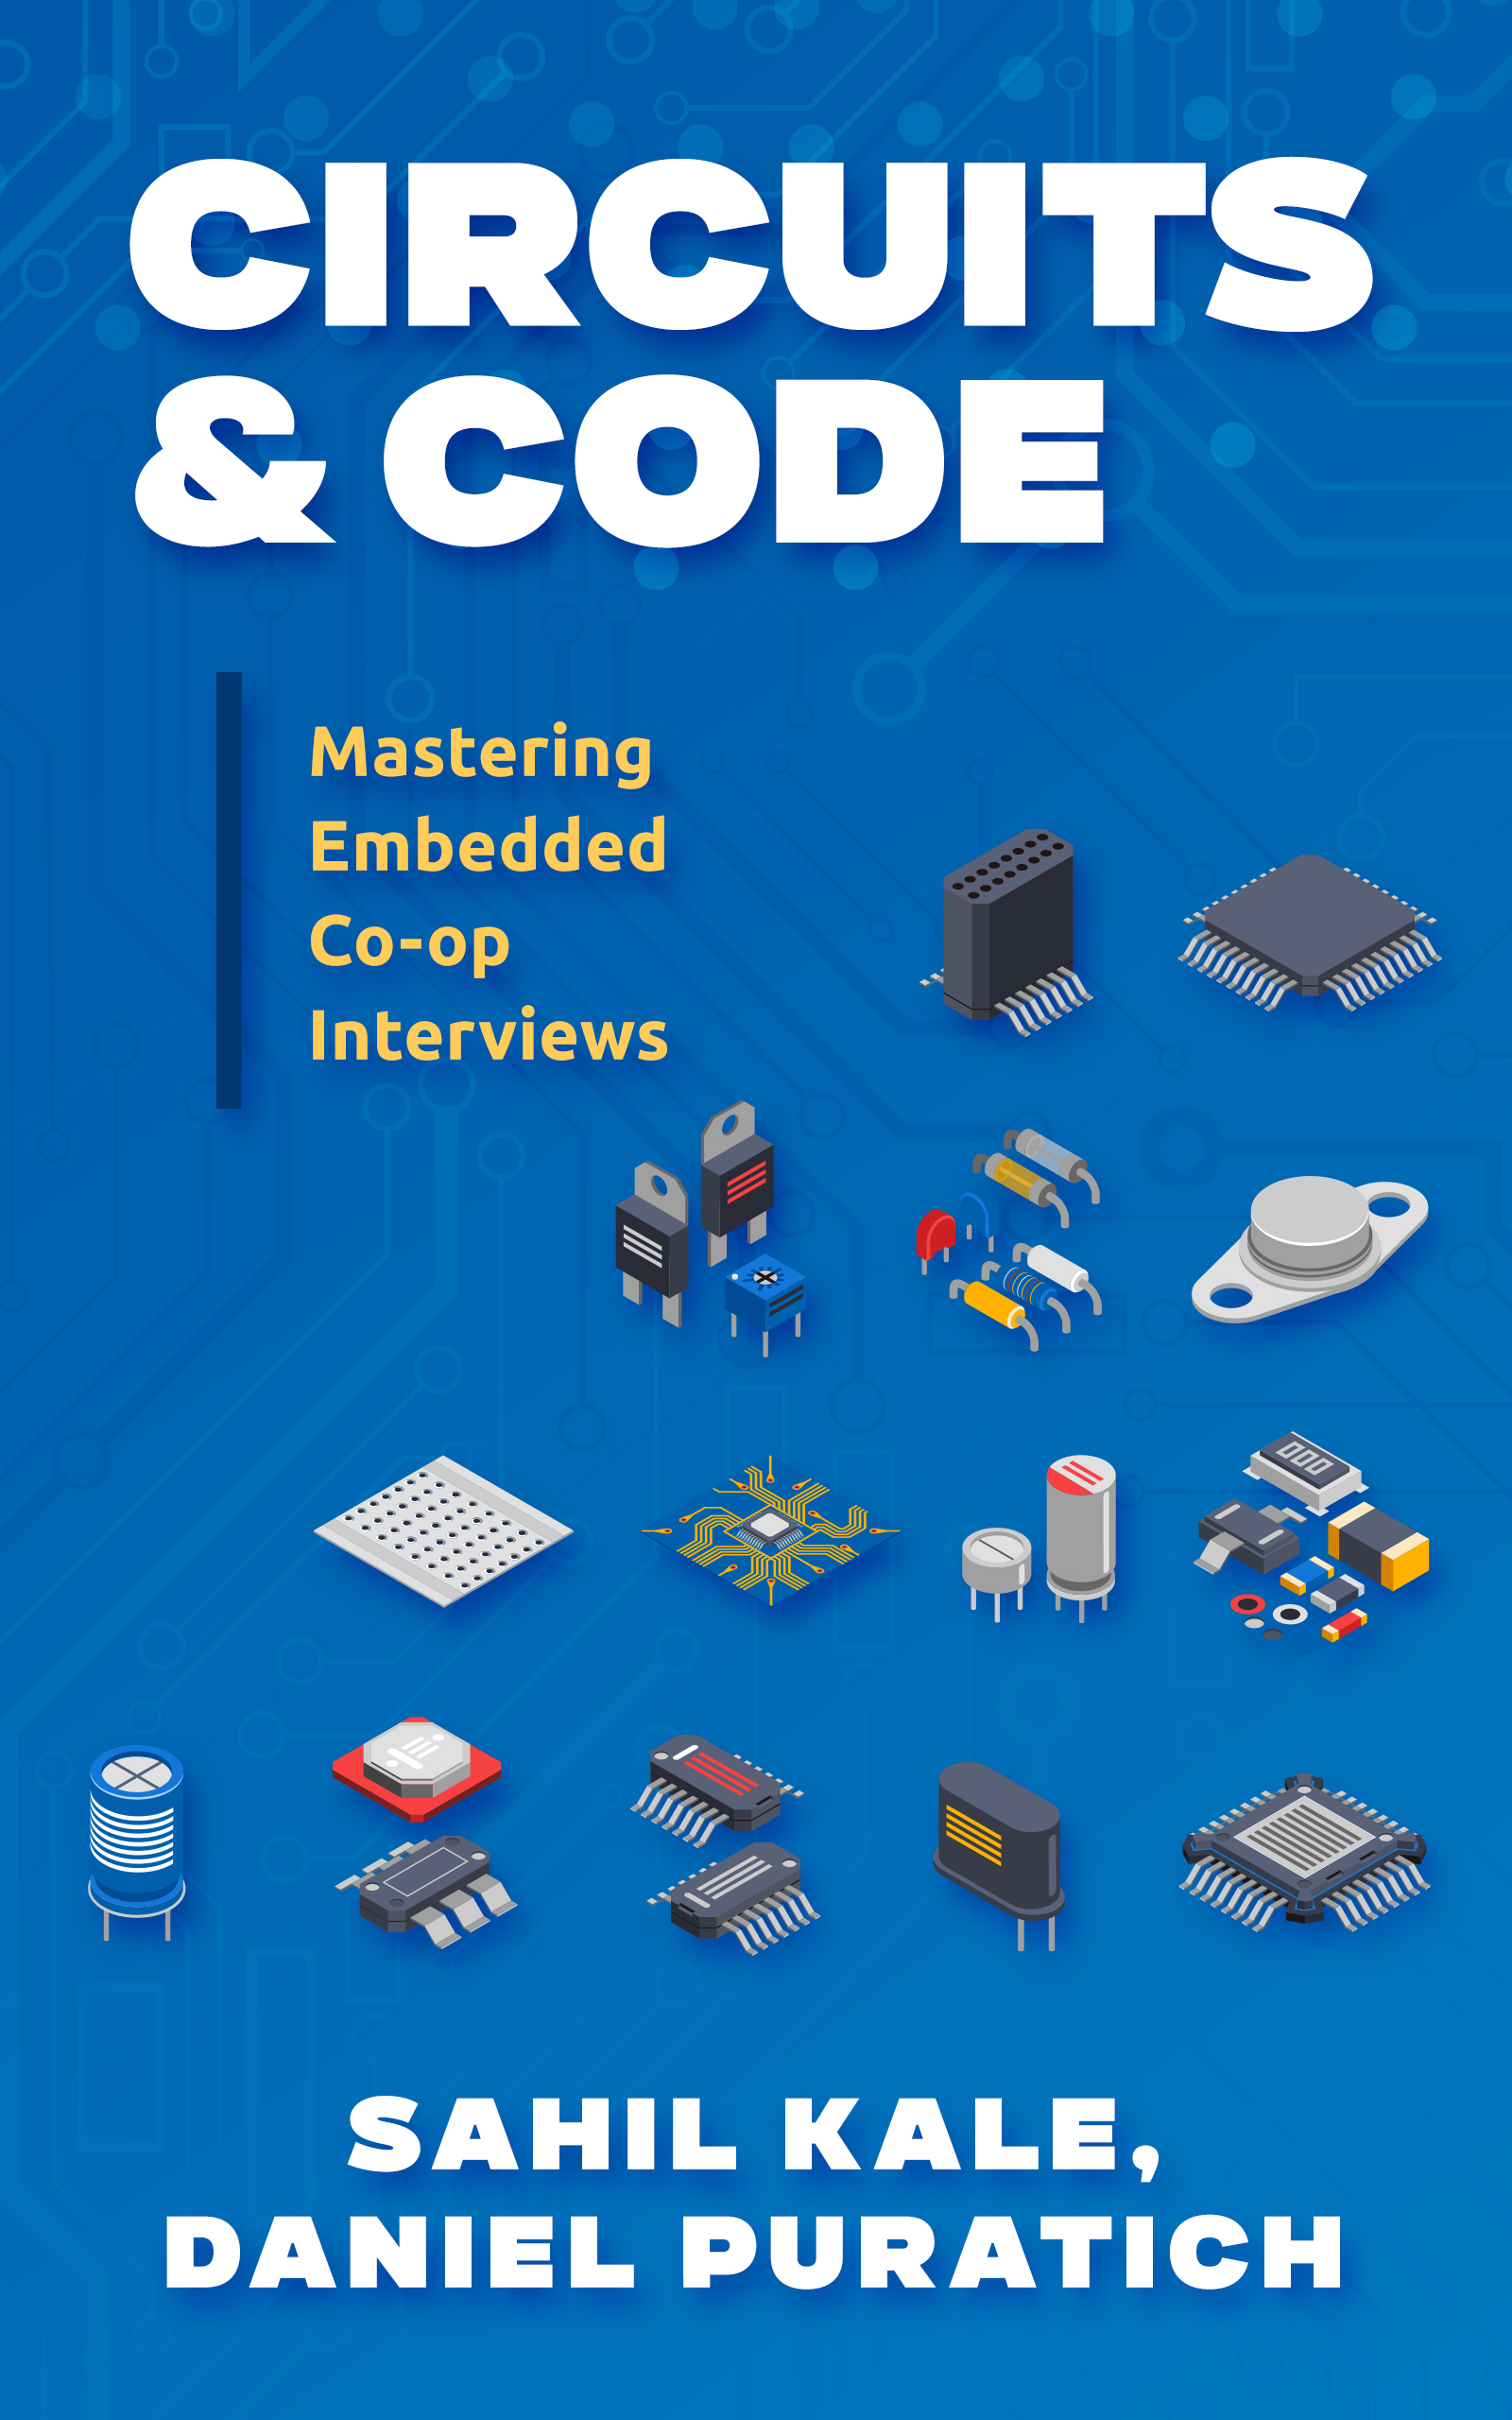
\includegraphics[width=0.8\textwidth]{images/cover.jpg}
\end{center}
\newpage

% Title Page
\title{Circuits \& Code: Mastering Embedded Co-op Interviews}
\author{\textcopyright \ Sahil Kale, Daniel Puratich}
% \date{} % By leaving this blank it defaults to the build date
\setlength{\droptitle}{0.3\textheight} % Moves the text down from the top
\maketitle % displays title, author, and build date field
\thispagestyle{empty} % Removes the page number on the title page
\newpage

\tableofcontents
\newpage

% One .tex per question (first edition is twenty questions, roughly three pages of solution each and one page for the question)
\subfile{preamble.tex}
\newpage
\subfile{bitstream_parity.tex}
\newpage
\subfile{voltage_divider.tex}
\newpage
\subfile{interrupts.tex}
\newpage
\subfile{led.tex}
\newpage
\subfile{keyword.tex} % place after interrupts.tex
\newpage
\subfile{signalling.tex}
\newpage
\subfile{pid.tex}
\newpage
\subfile{compare-i2c-spi.tex} % place after signalling.tex
\newpage
\subfile{spi-bitbang.tex} % place after compare-i2c-spi.tex
\newpage
\subfile{oscilloscope.tex} % place after voltage_divider.tex, signalling.tex
\newpage
\subfile{what-is-can.tex}
\newpage
\subfile{passives.tex} % place after voltage_divider.tex, oscilloscope.tex, signalling.tex, compare-i2c-spi.tex
\newpage
\subfile{packet-parsing.tex}
\newpage
\subfile{current_sense.tex}
\newpage
\subfile{adc_init.tex} 
\newpage
\subfile{64-bit-timer.tex}
\newpage
\subfile{stack-growth.tex}
\newpage
\subfile{opamp.tex}
\newpage
\subfile{mutex_vs_semaphore.tex}
\newpage
\subfile{buck_vs_ldo.tex} % place after passives.tex, opamp.tex
\newpage

% Appendix 
\subfile{appendix_packet_parsing_tests.tex}
\newpage
\subfile{appendix_switched_divider.tex}
\newpage
\subfile{appendix_more_passives.tex}
\newpage
\subfile{appendix_more _opamps.tex}
\newpage

% Bibliography
\printbibliography

\end{document}
